\begin{figure}[h]
	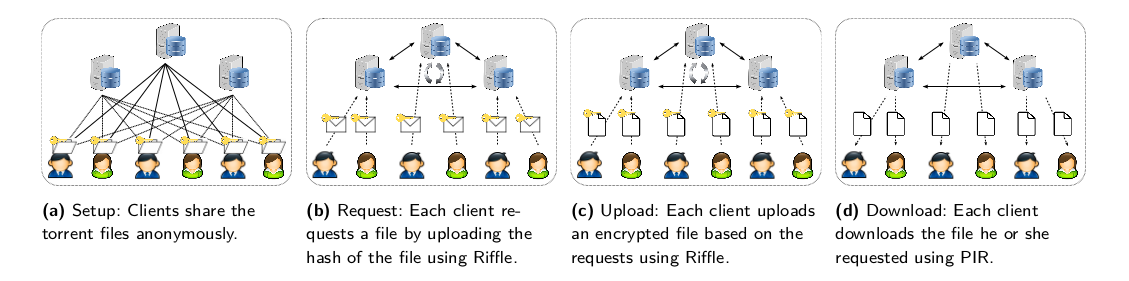
\includegraphics[scale=0.2]{anonymous.png}
	\caption{Protocolo de transferencia de archivos anónimo}
\end{figure}

\subsubsection{Protocolo de compartición de archivos}

La manera de compartir archivos en un grupo Riffle es similar a como lo hace BitTorrent, a pesar de las diferencias en el modelo (BitTorrent utiliza peer-to-peer y Riffle cliente-servidor). CUanod un cliente quiere compartir un archivo, genera un torrent, que contiene los hashes de todos los bloques del archivo. Entonces, usando Riffle, el cliente sube el torrent al servidor. Los servidores toman el papel de rastreador de torrentes en BitTorrent, y gestionan todos los archivos disponibles en el grupo. En el diseño más simple, los descriptores de archivo se difunden a todos los clientes conectados, y pueden elegir localmente un archivo para descargarlo. Dado que los torrent son suficientemente pequeños, incluso para archivos grandes, y compartirlos no es apenas costoso, asumimos que difundirlos no tiene ningún coste y nos centramos en compartir bloques. 

Con los torrents distribuídos, los clientes pueden ahora compartir de forma anónima los archivos usando Riffle. Este hecho se da en tres pasos:
\begin{enumerate}
	\item \textbf{Petición de bloques}. Cada $C_j$ identifica un archivo F de su interés y los hashes de los bloques del archivo $H_F$ a través del torrent. $C_j$ solicita un bloque de F subiendo el hash de dicho bloque a su servidor principal $S_{p_j}$ usando Riffle. Cuando un cliente no necesita requiere ningún bloque, manda un valor aleatorio como seña de que no quiere nada. Todas las peticiones $H_\pi$ se difunden a los clientes al final de este paso.
	\item \textbf{Subida de bloques.} Cada $C_j$ comprueba si tiene algún bloque mirando los hashes de los bloques que posee. Si encuentra alguno, entonces lo sube usando Riffle. Una vez que el texto plano del bloque está disponible para los servidores, cada servidor difunde los hashes $H'_\pi$ que tiene a su alcance a todos los clientes.
	\item \textbf{Descarga de bloques.} Desde $H_\pi$ y $H'_\pi$, $C_j$ conoce el índice del bloque pedido. Usando PIR, $C_j$ descarga el bloque. 
\end{enumerate}	

	Cada una de las peticiones son independientes, así que se pueden dar de forma paralela. En la figura 2 se resume el protocolo.

\subsubsection{Costes de banda ancha en la compartición de archivos}

Para compartir cada bloque entre usuarios en BitTorrent, cada cliente necesita solicitar y descargar un bloque. También podría necesitar subir un archivo si recibe una solicitud. Si cada solicitud tiene tamaño $h$, cada cliente consume $h+b$ de la banda ancha de subida y $b$ de la banda ancha de bajada. En Riffle con PIR, hay tres fuentes de costes de banda ancha por cliente: (1) descargar las peticiones, (2) subir los MACs de encriptación autenticada y (3) las máscaras para el servidor principal.  Por tanto, el total de banda ancha entre un cliente y un servidor es $h+b+n+2m \lambda$ de subida, y $b+2hn$ de bajada. Nótese que aunque la banda ancha necesaria crece con el número de clientes, $n$ y $2hn$ son mucho más pequeñas que $b$ en escenarios de compartición de archivos para un número razonable de clientes y de tamaño de archivo. 
